\chapter{Corriente continua}

\section{Enunciado}
Calcular las corrientes de malla mostradas en el circuito de la
figura.

\begin{center}
  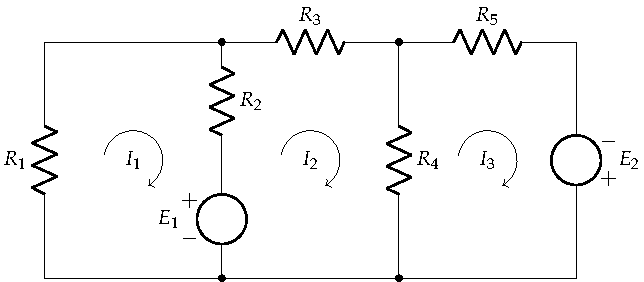
\includegraphics{figuras/BT1_02.pdf}
\end{center}

  \subsection*{Solución}
  Se plantea el sistema de ecuaciones en forma matricial:
  \begin{equation*}
    \begin{bmatrix}
      7 & -5 & 0 \\
      -5 & 19 & -4 \\
      0 & -4 & 6
    \end{bmatrix} \cdot
    \begin{bmatrix}
      I_1\\
      I_2\\
      I_3
    \end{bmatrix} = %
    \begin{bmatrix}
      -25 \\
      25\\
      50
    \end{bmatrix}
  \end{equation*}
  cuya solución es:
  \begin{align*}
    I_1&=\qty{-1.31}{\ampere}\\
    I_2&=\qty{3.17}{\ampere}\\
    I_3&=\qty{10.45}{\ampere}
  \end{align*}

  \noindent\rule{7in}{2.8pt}

%%%%%%%%%%%%%%%%%%%%%%%%%%%%%%%%%%%%%%%%%%%%%%%%%%%%%%%%%%%%%%%%%%%%%%%%%

  \section{Enunciado}
  Calcular el valor de $E$ que hace que $I_0=\qty{7.5}{\milli\ampere}$
  en el circuito de la figura.

  \begin{center}
    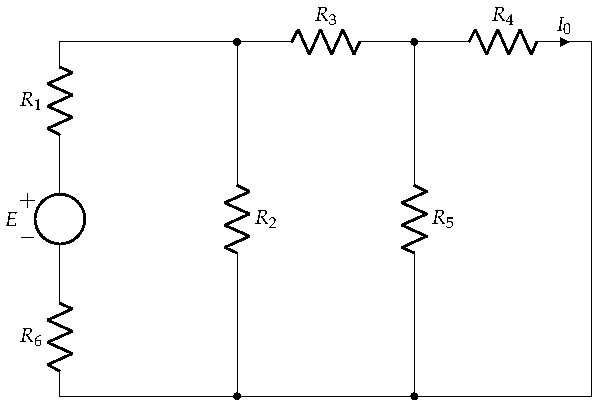
\includegraphics{figuras/BT1_03.pdf}
  \end{center}


\subsection*{Solución}
Se plantea el sistema de ecuaciones en forma matricial, suponiendo que
las tres mallas van en sentido horario:
\begin{equation*}
  \begin{bmatrix}
    27 & -7 & 0 \\
    -7 & 17 & -6 \\
    0 & -6 & 12
  \end{bmatrix} \cdot
  \begin{bmatrix}
    I_a\\
    I_b\\
    I_0
  \end{bmatrix} = %
  \begin{bmatrix}
    U_s \\
    0\\
    0
  \end{bmatrix}
\end{equation*}
donde además se sabe el valor de $I_0=\qty{7.5}{\milli\ampere}$. Por
tanto, de la tercera ecuación se puede obtener el valor de $I_b$:
\begin{equation*}
  -6\,I_b+12\,I_0=-6\,I_b+12\cdot 7.5 = 0\Rightarrow 6\,I_b=90 \Rightarrow I_b=\dfrac{90}{6}=\qty{15}{\milli\ampere}
\end{equation*}
Con $I_b$ calculado, se utiliza la segunda ecuación para determinar
$I_a$:
\begin{equation*}
  -7\,I_a+17\,I_b-6\,I_0=-7\,I_a+17\cdot 15-6\cdot 7.5 = 0\Rightarrow 7\,I_a=210\Rightarrow I_a=\dfrac{210}{7}=\qty{30}{\milli\ampere}
\end{equation*}
Determinada $I_a$, se emplea la primera ecuación para obtener el valor
de $U_s$:
\begin{equation*}
  27\,I_a-7\,I_b=27\cdot 30 - 7 \cdot 15 = U_s = {\qty{705}{\milli\volt}}
\end{equation*}

\noindent\rule{7in}{2.8pt}

%%%%%%%%%%%%%%%%%%%%%%%%%%%%%%%%%%%%%%%%%%%%%%%%%%%%%%%%%%%%%%%%%%%%%%%%%

\section{Enunciado}
Calcular la intensidad $I$ en el circuito de la figura.

\begin{center}
  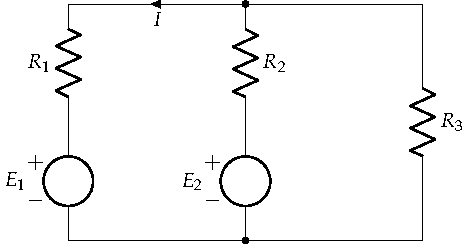
\includegraphics{figuras/BT1_04.pdf}
\end{center}


\subsection*{Solución}
Se suponen las mallas mostradas en la siguiente figura.

\begin{center}
  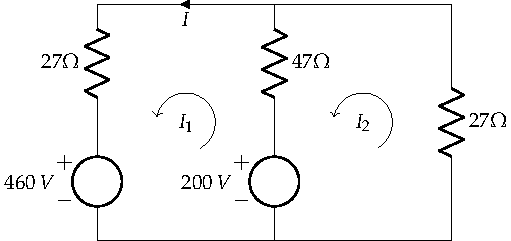
\includegraphics{figuras/BT1_04_mallas.pdf}
\end{center}

Se plantea el sistema de ecuaciones en forma matricial:
\begin{equation*}
  \begin{bmatrix}
    74 & -47  \\
    -47 & 74
  \end{bmatrix} \cdot
  \begin{bmatrix}
    I_1\\
    I_2
  \end{bmatrix} =
  \begin{bmatrix}
    -260 \\
    -200
  \end{bmatrix}
\end{equation*}
cuya solución es:
\begin{align*}
  I_1&=\qty{-8.77}{\ampere}\\
  I_2&=\qty{-8.27}{\ampere}
\end{align*}

%%%%%%%%%%%%%%%%%%%%%%%%%%%%%%%%%%%%%%%%%%%%%%%%%%%%%%%%%%%%%%%%%%
\section{Enunciado}
En el circuito de la figura obtener las intensidades de corriente
señaladas primero mediante un análisis por el método de las mallas y
posteriormente mediante un análisis por el método de los nudos.

\begin{center}
  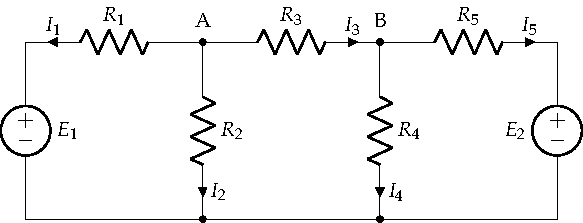
\includegraphics{figuras/BT1_08.pdf}
\end{center}

\subsection*{Solución}
Se aplica primero el método de las mallas, considerando las corrientes
de malla mostradas en la siguiente figura:
\begin{center}
  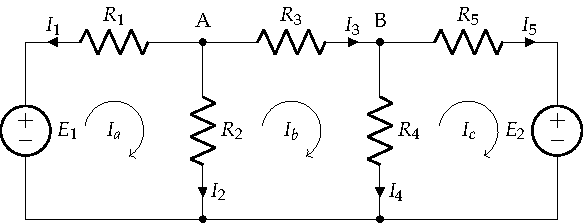
\includegraphics{figuras/BT1_08_mallas.pdf}
\end{center}

Se plantea el sistema de ecuaciones en modo matricial:
\begin{equation*}
  \begin{bmatrix}
    3 & -1 & 0 \\
    -1 & 10 & -5 \\
    0 & -5 & 8
  \end{bmatrix} \cdot
  \begin{bmatrix}
    I_a\\
    I_b\\
    I_c
  \end{bmatrix} = %
  \begin{bmatrix}
    10 \\
    0\\
    -6
  \end{bmatrix}
\end{equation*}
cuya solución es:
\begin{align*}
  I_a&=\qty{3.31}{\ampere}\\
  I_b&=\qty{-0.06}{\ampere}\\
  I_c&= \qty{-0.79}{\ampere}
\end{align*}
Se establecen las igualdades entre las diferentes corrientes de rama y
de malla, y se calculan sus valores:
\begin{align*}
  I_1&=-I_a=\qty{-3.31}{\ampere}\\
  I_2&=I_a-I_b=3.31-(-0.06)=\qty{3.37}{\ampere}\\
  I_3&=I_b=\qty{-0.06}{\ampere}\\
  I_4&=I_b-I_c=-0.06-(-0.79)=\qty{0.73}{\ampere}\\
  I_5&=I_c=\qty{-0.79}{\ampere}
\end{align*}
	
Para poder aplicar el método de los nudos, es necesario hacer, en
primer lugar, la transformación de las fuentes de tensión (y la
resistencia en serie) en fuentes de corriente (con una resistencia en
paralelo):
\begin{align*}
  I_{g,10V}&=\dfrac{\epsilon_{10V}}{R_{2\Omega}}=\dfrac{10}{2}=\qty{5}{\ampere}\\
  I_{g,6V}&=\dfrac{\epsilon_{6V}}{R_{3\Omega}}=\dfrac{6}{3}=\qty{2}{\ampere}
\end{align*}
quedando el circuito que se muestra a continuación.

\begin{center}
  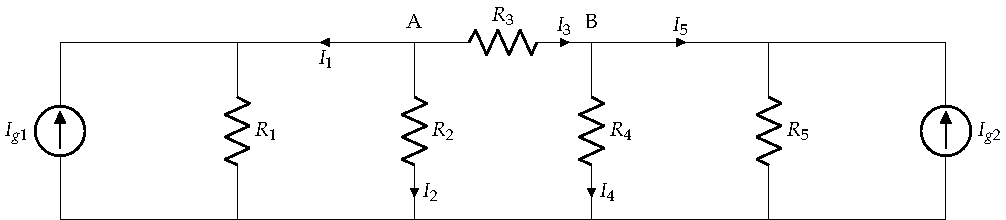
\includegraphics{figuras/BT1_08_nudos.pdf}
\end{center}

En este caso, se trabaja con las conductancias $G=\frac{1}{R}$. Se
escribe el sistema de ecuaciones en modo matricial:
\begin{equation*}
  \begin{bmatrix}
    1.75 & - 0.25\\
    -0.25 & 0.783
  \end{bmatrix} \cdot%
  \begin{bmatrix}
    U_A\\
    U_B
  \end{bmatrix} = %
  \begin{bmatrix}
    5\\
    2
  \end{bmatrix}
\end{equation*}
cuya solución es:
\begin{align*}
  U_A&=\qty{3.37}{\volt}\\
  U_B&=\qty{3.67}{\volt}
\end{align*}
Con estos valores, se pueden determinar directamente las corrientes
$I_2$ e $I_4$, por simple aplicación de la ley de Ohm:
\begin{align*}
  I_2&=\dfrac{U_A}{R_{1\Omega}}=\dfrac{3.37}{1}=\qty{3.37}{\ampere}\\
  I_4&=\dfrac{U_B}{R_{5\Omega}}=\dfrac{3.67}{5}=\qty{0.73}{\ampere}
\end{align*}
Las corrientes que circulan por las resistencias en paralelo con las
fuentes de tensión se determinan de manera análoga:
\begin{align*}
  I_{2\Omega}&=\dfrac{U_A}{R_{2\Omega}}=\dfrac{3.37}{2}=\qty{1.69}{\ampere}\\
  I_{3\Omega}&=\dfrac{U_B}{R_{3\Omega}}=\dfrac{3.67}{3}=\qty{1.22}{\ampere}
\end{align*}
Por la 1LK, se determina el valor de $I_1$, $I_3$ e $I_5$:
\begin{align*}
  I_1&+5=I_{2\Omega}\Rightarrow I_1=I_{2\Omega}-5=1.69-5=\qty{-3.31}{\ampere}\\
  I_5&+2=I_{3\Omega}\Rightarrow I_5=I_{3\Omega}-2=1.22-2=\qty{-0.78}{\ampere}\\
  I_3&=I_4+I_5=0.73+(-0.78)=\qty{-0.05}{\ampere}
\end{align*}

Se observa que los resultados obtenidos con ambos métodos son
idénticos.

%%%%%%%%%%%%%%%%%%%%%%%%%%%%%%%%%%%%%%%%%%%%%%%%%%%%%%%%%%%%%%%%%%
\section{Enunciado}
Analizar el circuito de la figura mediante el método de las mallas,
obteniendo la corriente de cada una de las ramas. Con este resultado,
calcular la diferencia de potencial entre A y B, y realizar un balance
de potencias comparando la potencia de los elementos activos y la de
los elementos pasivos.

Datos:
$R_1 = R_2 = \qty{1}{\ohm}; R_3 = \qty{2}{\ohm}; R_4 = \qty{3}{\ohm};
R_5=\qty{4}{\ohm}; \epsilon_1=\qty{118}{\volt}; \epsilon_2 =
\qty{236}{\volt}; \epsilon_3 = \qty{118}{\volt}$.

\begin{center}
  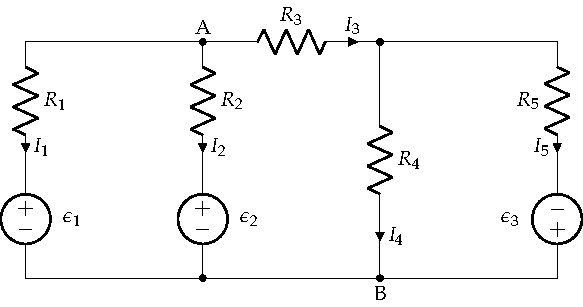
\includegraphics{figuras/mallas2.pdf}
\end{center}

\subsection*{Solución}
Se usan tres corrientes de malla con giro a derechas, de nombre (de
izquierda a derecha), $I_a$, $I_b$ e $I_c$. Escribiendo el sistema de
ecuaciones del método de las mallas en forma matricial:
\begin{equation*}
  \begin{bmatrix}
    2 & -1 & 0 \\
    -1 & 6 & -3 \\
    0 & -3 & 7
  \end{bmatrix}
  \cdot
  \begin{bmatrix}
    I_a\\
    I_b\\
    I_c
  \end{bmatrix}
  =
  \begin{bmatrix}
    -118\\
    236\\
    118
  \end{bmatrix}
\end{equation*}
cuya solución es:
\begin{align*}
  I_a &= \qty{-32}{\ampere}\\
  I_b &= \qty{54}{\ampere}\\
  I_c &= \qty{40}{\ampere}
\end{align*}

Estableciendo las relaciones entre las corrientes de rama y las
corrientes de malla, y sustituyendo, se llega a la conclusión de que:

\begin{align*}
  I_1 &= -I_a=\qty{32}{\ampere}\\
  I_2 &= I_a - I_b=-32-54=\qty{-86}{\ampere}\\
  I_3 &= I_b=\qty{54}{\ampere}\\
  I_4 &= I_b - I_c=54-40=\qty{14}{\ampere}\\
  I_5 &= I_c=\qty{40}{\ampere}
\end{align*}

\emph{Se recomienda comprobar que estos resultados cumplen la 1LK en
  los nudos del circuito, para asegurarse de que la resolución es
  correcta.}

La diferencia de potencial entre A y B es:
\begin{equation*}
  U_{AB} = I_3 \cdot R_3 + I_4 \cdot R_4 = 54\cdot 2+14\cdot 3= \qty{150}{\volt}
\end{equation*}

Para hacer el balance de potencias:
\begin{itemize}
\item \textbf{Potencia de los generadores:}
  \begin{itemize}
  \item $P_{\epsilon1}=\epsilon_1\,I_1=118\cdot 32=\qty{3776}{\watt}$
  \item
    $P_{\epsilon2}=\epsilon_2\,I_2=236\cdot (-86)=\qty{-20296}{\watt}$
  \item
    $P_{\epsilon3}=-\epsilon_3\,I_3=-118\cdot 40=\qty{-4720}{\watt}$
  \end{itemize}
\item \textbf{Potencia de las resistencias:}
  \begin{itemize}
  \item $P_{R,1}=R_1\,I_1^2=1\cdot 32^2=\qty{1024}{\watt}$
  \item $P_{R,2}=R_2\,I_2^2=1\cdot (-86)^2=\qty{7396}{\watt}$
  \item $P_{R,3}=R_3\,I_3^2=2\cdot 54^2=\qty{5832}{\watt}$
  \item $P_{R,4}=R_4\,I_4^2=3\cdot 14^2=\qty{588}{\watt}$
  \item $P_{R,5}=R_5\,I_5^2=4\cdot 40^2=\qty{6400}{\watt}$
  \end{itemize}
\end{itemize}
donde se cumple que la suma es igual a 0.

%%%%%%%%%%%%%%%%%%%%%%%%%%%%%%%%%%%%%%%%%%%%%%%%%%%%%%%%%%%%%%%%%%
\section{Enunciado}
En el circuito de la figura, determinar:
\begin{itemize}
\item Todas las intensidades de rama señaladas
\item Carga, polaridad y energía almacenada en los condensadores
\item Balance de potencias
\end{itemize}

\begin{center}
  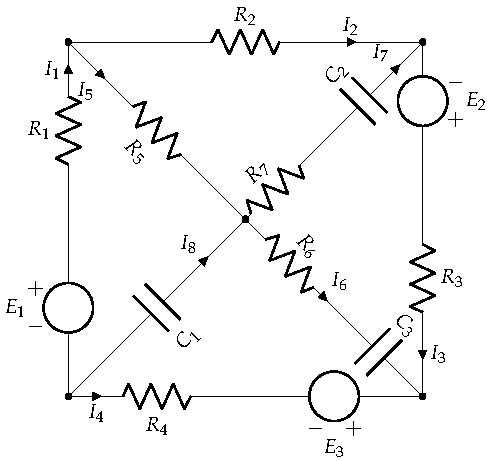
\includegraphics{figuras/BT1_09.pdf}
\end{center}

\subsection*{Solución}
Al tratarse de un circuito alimentado por corriente continua, los
condensadores se comportan como un circuito abierto, por lo que el
circuito a analizar es el mostrado en la figura.

\begin{center}
  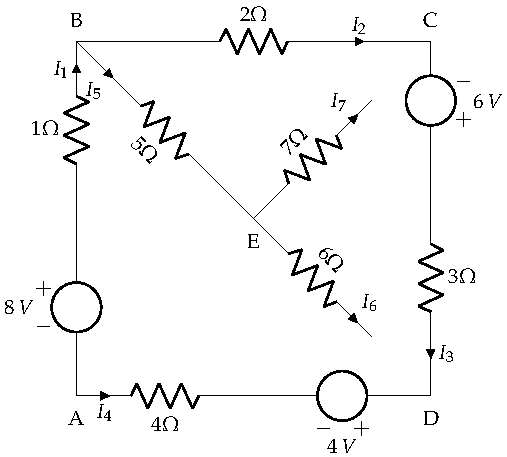
\includegraphics{figuras/BT1_09_sol.pdf}
\end{center}

Por simple observación, obtenemos:
\begin{equation*}
  I_5=I_6=I_7=\qty{0}{\ampere}
\end{equation*}
quedando una única malla por la que circula la misma corriente
$I_1=I_2=I_3=I_4=I$. Por la 2LK, considerando que $I$ va en sentido
horario, se obtiene que:
\begin{equation*}
  -8+1\, I+2\,I-6+3\,I+4+4\,I=0\Rightarrow {I = \dfrac{8+6-4}{1+2+3+4}=\qty{1}{\ampere}=I_1=I_2=I_3=-I_4}
\end{equation*}

Para determinar la carga de los condensadores hay que calcular las
tensiones en los diferentes nudos. Considerando $E$ como tierra:
\begin{align*}
  U_{AE}&=U_{A}-\cancelto{0}{U_{E}}=-8+1\,I_1+5\,I_5=-8+1\cdot 1 + 5\cdot 0=\qty{-7}{\volt}\\
  U_{CE}&=U_{C}-\cancelto{0}{U_{E}}=-2\,I_2+5\,I_5=-2\cdot 1+5\cdot 0 =\qty{-2}{\volt}\\
  U_{DE}&=U_{D}-\cancelto{0}{U_{E}}=4-4\, I_4-8+1\,I_1+5\,I_5=4-4\cdot (-1)-8+1\cdot 1 +5\cdot 0=\qty{1}{\volt}
\end{align*}
Con estas tensiones, se determina la carga de los condensadores:
\begin{align*}
  Q_{1\mu F}&=C_{1\mu F}\, U_{AE} = 1\cdot 10^{-6}\cdot (-7)=\qty{-7}{\micro\coulomb}\\
  Q_{2\mu F}&=C_{2\mu F}\, U_{CE} = 2\cdot 10^{-6}\cdot (-2)=\qty{-4}{\micro\coulomb}\\
  Q_{3\mu F}&=C_{3\mu F}\, U_{DE} = 3\cdot 10^{-6}\cdot 1=\qty{3}{\micro\coulomb}
\end{align*}
Aquellos condensadores en los que la carga es negativa, significa que
tienen la polaridad contraria a la considerada. La energía es:
\begin{align*}
  E_{1\mu F}&=\dfrac{1}{2}\,C_{1\mu F}\cdot U_{AE}^2 = \dfrac{1}{2}\cdot 1\cdot 10^{-6}\cdot (-7)^2=24.5\,\mu\text{J}\\
  E_{2\mu F}&=\dfrac{1}{2}\,C_{2\mu F}\cdot U_{CE}^2 = \dfrac{1}{2}\cdot 2\cdot 10^{-6}\cdot (-2)^2=4\,\mu\text{J}\\
  E_{3\mu F}&=\dfrac{1}{2}\,C_{3\mu F}\cdot U_{DE}^2 = \dfrac{1}{2}\cdot 3\cdot 10^{-6}\cdot 1^2=1.5\,\mu\text{J}
\end{align*}

Se calculan las potencias generadas y consumidas por las resistencias:
\begin{itemize}
\item \textbf{Potencias generadas:}
  \begin{itemize}
  \item Generador 8 V: $P_{g,8V}=-U_{8V}\,I_1=-8\cdot 1=-8$ W
  \item Generador 6 V: $P_{g,6V}=-U_{6V}\,I_3=-6\cdot 1=-6$ W
  \end{itemize}
\item \textbf{Potencias consumidas:}
  \begin{itemize}
  \item Generador 4 V: $P_{g,4V}=-U_{4V}\,I_4=-4\cdot (-1)=4$ W
  \item Resistencia 1$\Omega$: $P_{R,1}=R_1\,I_1^2=1\cdot 1^2=1$ W
  \item Resistencia 2$\Omega$: $P_{R,2}=R_2\,I_2^2=2\cdot 1^2=2$ W
  \item Resistencia 3$\Omega$: $P_{R,3}=R_3\,I_3^2=3\cdot 1^2=3$ W
  \item Resistencia 4$\Omega$: $P_{R,4}=R_4\,I_4^2=4\cdot (-1)^2=4$ W
  \end{itemize}
\end{itemize}
donde se cumple que la suma es 0.

%%%%%%%%%%%%%%%%%%%%%%%%%%%%%%%%%%%%%%%%%%%%%%%%%%%%%%%%%%%%%%%%%% 

\section{Enunciado}
Aplicar el método de los nudos en el circuito de la figura para
determinar:
\begin{itemize}
\item Los potenciales de los nudos A, B, C y D.
\item Las intensidades de corriente señaladas.
\item Carga, polaridad y energía almacenada en los condensadores,
  supuestos sin carga inicial.
\end{itemize}
Datos:
$R_i = \mathrm{i\ } \Omega; C_i = \mathrm{i\ } \mu F; E_1 = 6V; E_2 =
18 V; E_3 = {6} V$

\begin{center}
  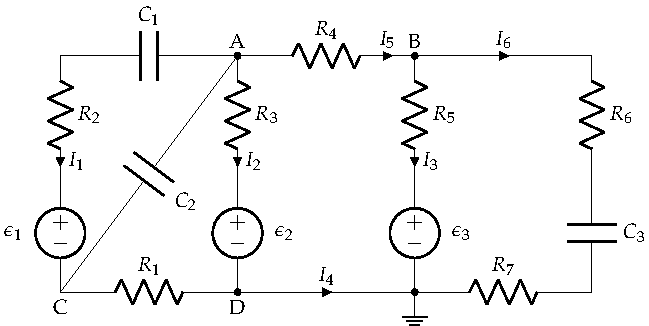
\includegraphics[]{figuras/nudos_condensadores.pdf}
\end{center}

\subsection*{Solución}
Se sustituyen los condensadores por circuitos abiertos. En
consecuencia, por las ramas correspondientes no puede circular
corriente:
\begin{align*}
  I_1 &= 0A\\
  I_6 &= 0 A
\end{align*}

Para aplicar el método de los nudos transformamos las fuentes
$\epsilon_2$ y $\epsilon_3$ en fuentes de corriente, de valor:
\begin{align*}
  I_{\epsilon2}&=\dfrac{\epsilon_2}{R_3}=\dfrac{18}{3}=\qty{6}{\ampere}\\
  I_{\epsilon3}&=\dfrac{\epsilon_3}{R_5}=\dfrac{6}{5}=\qty{1.2}{\ampere}
\end{align*}
Se plantea el método de los nudos en forma matricial:
\begin{equation*}
  \begin{bmatrix}
    \frac{1}{3} + \frac{1}{4} & -\frac{1}{4}\\
    -\frac{1}{4} & \frac{1}{5} + \frac{1}{4}
  \end{bmatrix} \cdot %
  \begin{bmatrix}
    U_A\\
    U_B
  \end{bmatrix} = %
  \begin{bmatrix}
    6\\
    1.2
  \end{bmatrix}
\end{equation*}
Resolviendo el sistema:
\begin{align*}
  U_A &= {15}V\\
  U_B &= {11} V
\end{align*}
Además, puesto que $D$ está conectado a tierra:
\begin{equation*}
  {U_D = 0 V}
\end{equation*}
Por otra parte, la caída de tensión en la resistencia $R_1$ es 0
porque $I_1 = 0$, luego:
\begin{equation*}
  {U_C = U_D=0 V}
\end{equation*}
Con estos resultados se pueden obtener los valores de las corrientes
de rama:

\begin{align*}
  U_A&= I_2 \cdot R_3 + \epsilon_2\Rightarrow I_2=\dfrac{15-18}{3}={-1 A}\\
  U_B& = I_3 \cdot R_5 + \epsilon_3\Rightarrow I_3=\dfrac{11-6}{5}={1 A}
\end{align*}

Además, teniendo en cuenta que $I_1 = I_6 = 0$, se obtiene:
\begin{align*}
  I_5 &= I_3=1A\\
  I_4 &= I_2=-1 A
\end{align*}

Finalmente, se calculan las diferencias de potencial en los
condensadores. Para $C_1$, se considera la polaridad positiva en A:
\begin{equation*}
  U_{AC} = U_{C1} + \epsilon_1 \Rightarrow U_{C1} = 15-6= {{9} V}
\end{equation*}

Para $C_2$ y $C_3$ el cálculo es directo, asignando la polaridad
positiva en A y B, respectivamente:
\begin{equation*}
  U_{C2} =  U_{AC} = {{15} V}
\end{equation*}
\begin{equation*}
  U_{C3} =  U_{BD} = {{11} V}
\end{equation*}
  

En consecuencia, las cargas almacenadas en cada condensador son:
\begin{align*}
  q_1 &= C_1 \cdot U_{C1} = {{9}{\mu C}}\\
  q_2&= C_2 \cdot U_{C2} = {{30}{\mu C}}\\
  q_3 &= C_3 \cdot U_{C3} = {{33}{\mu C}}
\end{align*}
  
Y las energías:
\begin{align*}
  E_{C1} &= \frac{1}{2} \cdot C_1 \cdot U^2_{C1} = {{40.5}{\mu J}}\\
  E_{C2} &= \frac{1}{2} \cdot C_2 \cdot U^2_{C2} = {{225}{\mu J}}\\
  E_{C3} &= \frac{1}{2} \cdot C_3 \cdot U^2_{C3} = {{181.5}{\mu J}}
\end{align*}
  
%%%%%%%%%%%%%%%%%%%%%%%%%%%%%%%%%%%%%%%%%%%%%%%%%%%%%%%%%%%%%%%%%%

\section{Enunciado}

En el circuito de la figura, donde se sabe que la carga inicial de los
condensadores era de $\qty{10}{\micro\coulomb}$ para $C_1$ y de
$\qty{20}{\micro\coulomb}$ para $C_2$ con las polaridades indicadas,
se pide determinar:
\begin{itemize}
\item Intensidades de corriente señaladas
\item Potenciales en los puntos A, B, C, D, E y F
\end{itemize}

Datos:
$\epsilon_{A}=\SI{90}{\volt};\quad \epsilon_{B}=\SI{60}{\volt};\quad
\epsilon_{C}=\SI{30}{\volt};\quad R_{1}= R_2 = R_3 =
\SI{10}{\ohm};\quad R_{4}= R_5 = \SI{30}{\ohm};\quad C_{1}=
\SI{10}{\micro\farad};\quad C_{2}= \SI{20}{\micro\farad};\quad L_1 =
\SI{1}{\micro\henry}$

\begin{center}
  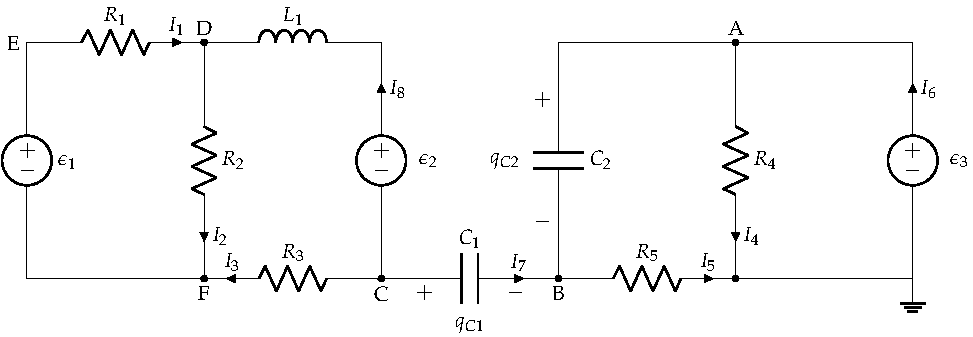
\includegraphics[scale = 0.8]{figuras/mallas_carga_inicial.pdf}
\end{center}


\subsection*{Solución}
Al estar alimentado por corriente continua, los condensadores se
comportan como un circuito abierto, y la bobina como un cortocircuito,
quedando el circuito como el mostrado en la figura. Se puede afirmar
que:
\begin{align*}
  {I_5=0A}\\
  {I_7=0A}
\end{align*}

\begin{center}
  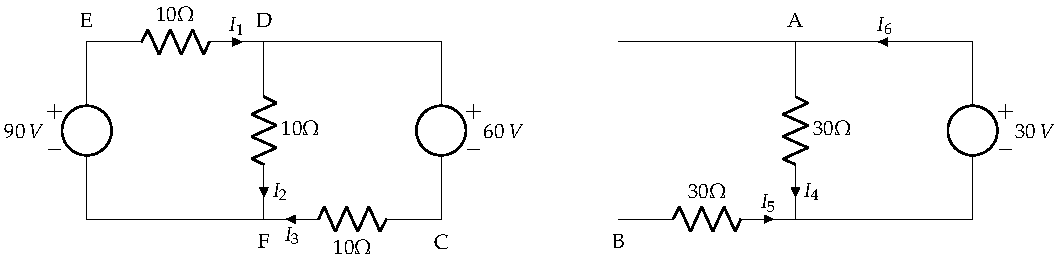
\includegraphics[width=\linewidth]{figuras/BT1_10_mod.pdf}
\end{center}

En el circuito de la izquierda se tienen dos mallas, considerando las
corrientes mostradas en la figura.

\begin{center}
  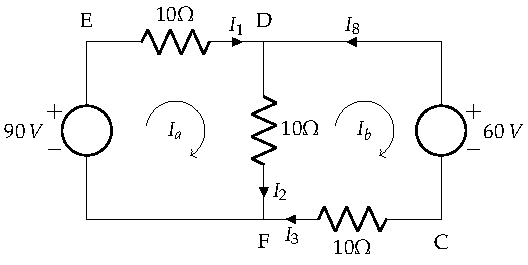
\includegraphics{figuras/BT1_10_izq_mallas.pdf}
\end{center}

Se plantea el sistema de ecuaciones en modo matricial:
\begin{equation*}
  \begin{bmatrix}
    20 & -10 \\
    -10 & 20
  \end{bmatrix} \cdot
  \begin{bmatrix}
    I_a\\
    I_b
  \end{bmatrix} = %
  \begin{bmatrix}
    90 \\
    -60
  \end{bmatrix}
\end{equation*}
cuya solución es:
\begin{align*}
  I_a&=\qty{4}{\ampere}\\
  I_b&=\qty{-1}{\ampere}
\end{align*}
Se establecen las igualdades entre las diferentes corrientes de rama y
de malla, y se calculan sus valores:
\begin{align*}
  I_1&=I_a=\qty{4}{\ampere}\\
  I_2&=I_a-I_b=4-(-1)=\qty{5}{\ampere}\\
  I_3&=I_b=\qty{-1}{\ampere}\\
  I_8&=-I_b=-(-1)=\qty{1}{\ampere}
\end{align*}
	
Para el circuito de la derecha se tiene una única malla:
\begin{equation*}
  {I_4=I_6=\dfrac{U_{30V}}{R_{30\Omega}}=\dfrac{30}{30}=\qty{1}{\ampere}}
\end{equation*}

Los potenciales en los puntos $A$ y $B$ son:
\begin{equation*}
  {U_A = \epsilon_C = {30} V}
\end{equation*}
\begin{equation*}
  U_B = R_5 \, I_5 = {0} V
\end{equation*}
Para calcular el potencial en el punto $C$ se debe tener en cuenta que
el condensador $C_1$ conserva su carga inicial porque el circuito no
está cerrado en la parte superior. Por tanto,
\begin{equation*}
  U_{CB} = U_{C1} = \dfrac{q^0_{C1} }{C_1} =\dfrac{10}{10}= {1 V}
\end{equation*}
Por tanto,
\begin{equation*}
  U_C = U_{CB} + U_B = 1+0={{1} V}
\end{equation*}

A partir de este resultado, se calculan el resto de potenciales:

\begin{align*}
  U_D &= U_{DC} + U_C = \epsilon_B + U_C =60+1={{61} V}\\
  U_E &= U_{ED} + U_D = I_1 \, R_1 + U_D =4\cdot 10+61={{101} V}\\
  U_F &= U_{FC} + U_C = -I_3 \, R_3 + U_C =-(-1)\cdot 10+1={{11} V}
\end{align*}

%%%%%%%%%%%%%%%%%%%%%%%%%%%%%%%%%%%%%%%%%%%%%%%%%%%%%%%%%%%%%%%%%% 
\section{Enunciado}
En el circuito de la figura, los condensadores se conectaron sin
carga. Mediante el método de las mallas determina:
\begin{itemize}
\item Intensidades de corriente señaladas
\item Potenciales en los puntos A, B, C y D
\item Polaridades, cargas, y energías de los condensadores
\item Balance de potencias
\end{itemize}
Datos:
$ \epsilon_{1}={118}V; \epsilon_{2}={236} V; \epsilon_{3}=118V; R_{1}=
{4}\Omega; R_{2}=R_{3}={1}{\Omega}; R_{4}= {3}{\Omega};
R_{5}={2}{\Omega}; C_{1}=C_{2}=C_{3}={2}{\mu F}; X_1 = X_2 = X_3 =
{1}{\Omega}$

\begin{center}
  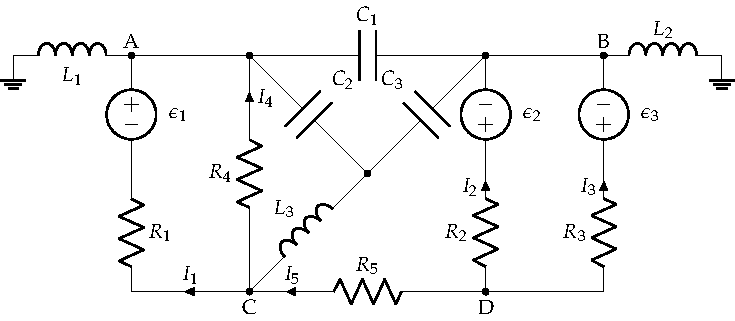
\includegraphics{figuras/mallas_condensadores.pdf}
\end{center}

\subsection*{Solución}
Se sustituyen los condensadores y las bobinas por sus equivalentes en
un circuito de corriente continua (circuito abierto y cortocircuito,
respectivamente). En el circuito resultante se marcan tres corrientes
de malla como se muestra en el circuito de la figura.

\begin{center}
  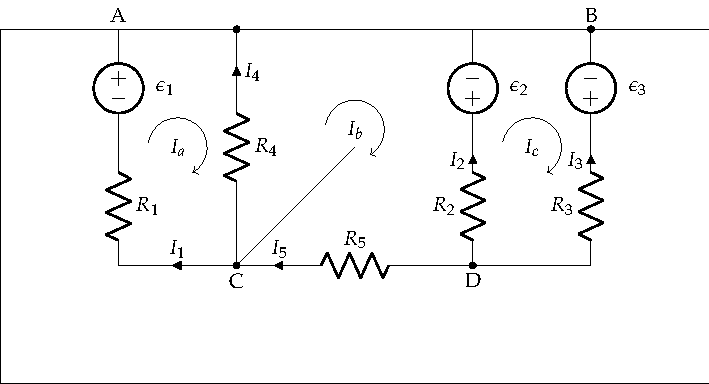
\includegraphics{figuras/mallas_condensadores_sol.pdf}
\end{center}

Planteando el sistema de ecuaciones en forma matricial:

\begin{equation*}
  \begin{bmatrix}
    7 & -3 & 0\\
    -3 & 6 & -1\\
    0 & -1 & 2
  \end{bmatrix}
  \cdot
  \begin{bmatrix}
    I_a\\
    I_b\\
    I_c
  \end{bmatrix}
  =
  \begin{bmatrix}
    118\\
    236\\
    -118
  \end{bmatrix}
\end{equation*}

La solución es:
\begin{align*}
  I_a & =  {40}A\\
  I_b & =  {54}A\\
  I_c & =  -{32}A
\end{align*}

Por tanto, las corrientes indicadas en el circuito son:

\begin{align*}
  I_1 &= I_a =  {40}A\\
  I_2  &= I_c-I_b =-32-54= {-86}A\\
  I_3  &= -I_c=  {32}A\\
  I_4& = I_b-I_a = 54-40=  {14}A\\
  I_5 &= I_b=  {54}A
\end{align*}


Las tensiones en los puntos indicados son:
\begin{align*}
  U_A&=U_B = {0}V\\
  U_C &= I_4 \cdot R_4 =14\cdot 3= {42}V\\
  U_D &= I_5 \cdot R_5 + U_C = 54\cdot 2+42= {150}V
\end{align*}

Por tanto, suponiendo como polaridad $+$ los extremos de los
condensadores $C_1$ y $C_2$ conectados a $A$, y el $C_3$ conectado a
$B$, los valores de tensión son:
\begin{align*}
  U_{C1} &= U_{AB} =  {0}V\\
  q_1 &= C_1 \cdot U_{C1}  = 0 \mu F\\
  E_{C1} &=\frac{1}{2} \cdot C_1 \cdot U^2_{C1} = {0}J
\end{align*}

\begin{align*}
  U_{C2} &= U_{AC} =  0-42=-42V \text{ (polaridad opuesta)}\\
  q_2 &= C_2 \cdot U_{C2} = 2\cdot 42 = 84 \mu F\\
  E_{C2} &=\frac{1}{2} \cdot C_2 \cdot U^2_{C2} = \frac{1}{2} \cdot 84\cdot 10^{-6} \cdot 42^2=1.76 mJ
\end{align*}

\begin{align*}
  U_{C3} &= U_{BC} =  0-42=-42V \text{ (polaridad opuesta)}\\
  q_3 &= C_3 \cdot U_{C3} = 2\cdot 42 = 84 \mu F\\
  E_{C3} &=\frac{1}{2} \cdot C_3 \cdot U^2_{C3} = \frac{1}{2} \cdot 84\cdot 10^{-6} \cdot 42^2=1.76 mJ
\end{align*}

Finalmente, el balance de potencias calcula la potencia entregada por
los elementos activos y la potencia consumida por los elementos
pasivos.
\begin{itemize}
\item \textbf{Potencia de los generadores:}
  \begin{itemize}
  \item $P_{\epsilon1}=-\epsilon_1\,I_1=-118\cdot 40=-4720$ W (G)
  \item $P_{\epsilon2}=\epsilon_2\,I_2=236\cdot (-86)=-20296$ W (G)
  \item $P_{\epsilon3}=\epsilon_3\,I_3=118\cdot 32=3776$ W (R)
  \end{itemize}
\item \textbf{Potencia de las resistencias:}
  \begin{itemize}
  \item $P_{R1}=R_1\,I_1^2=4\cdot 40^2=6400$ W
  \item $P_{R2}=R_2\,I_2^2=1\cdot (-86)^2=7396$ W
  \item $P_{R3}=R_3\,I_3^2=1\cdot 32^2=1024$ W
  \item $P_{R4}=R_4\,I_4^2=3\cdot 14^2=588$ W
  \item $P_{R5}=R_5\,I_5^2=2\cdot 54^2=5832$ W
  \end{itemize}
\end{itemize}
donde se cumple que la suma es 0.

%%%%%%%%%%%%%%%%%%%%%%%%%%%%%%%%%%%%%%%%%%%%%%%%%%%%%%%%%%%%%%%%%% 
\section{Enunciado}
En el circuito de la figura, determinar:
\begin{itemize}
\item Las ecuaciones para el cálculo de las intensidades
\item Todas las intensidades indicadas
\item Potenciales en todos los nudos
\item Carga y energía almacenada en los condensadores
\end{itemize}

\begin{center}
  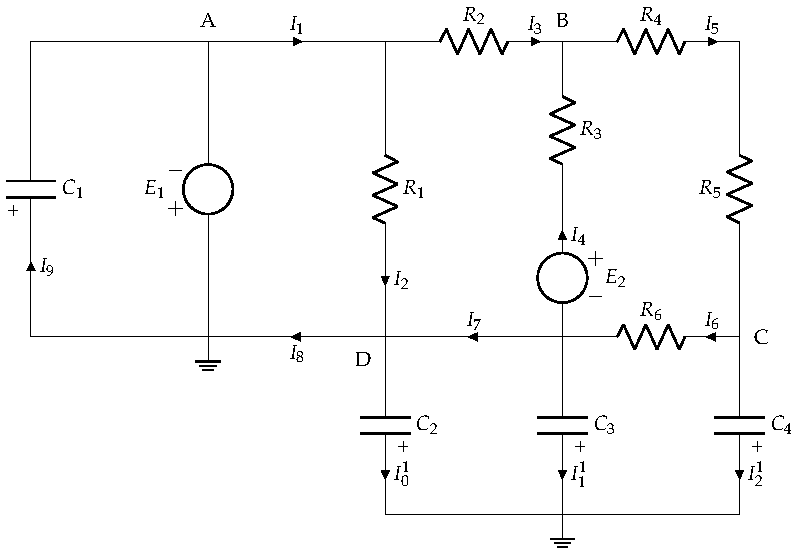
\includegraphics{figuras/BT1_11.pdf}
\end{center}


\subsection*{Solución}
Al tratarse de alimentación en CC, se sustituyen los condensadores por
circuitos abiertos, quedando el circuito de la figura:
\begin{center}
  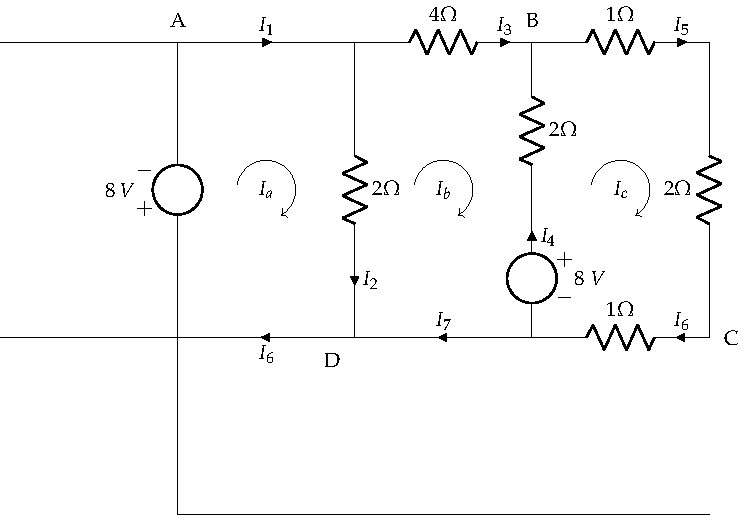
\includegraphics{figuras/BT1_11_mod.pdf}
\end{center}

Aplicando el método de mallas, con las corrientes indicadas, se
plantea el sistema de ecuaciones en forma matricial:
\begin{equation*}
  \begin{bmatrix}
    2 & -2 & 0 \\
    -2 & 8 & -2 \\
    0 & -2 & 6
  \end{bmatrix} \cdot
  \begin{bmatrix}
    I_a\\
    I_b\\
    I_c
  \end{bmatrix} = %
  \begin{bmatrix}
    -8 \\
    -8\\
    8
  \end{bmatrix}
\end{equation*}
Las ecuaciones completas para calcular las intensidades son:
\begin{align*}
  2\,I_a&-2\,I_b = -8\\
  -2\,I_a&+8\,I_b-2\,I_c = -8\\
  -2\,I_b&+ 6\,I_c = 8
\end{align*}
cuya solución es:
\begin{align*}
  I_a&=\qty{-6.5}{\ampere}\\
  I_b&=\qty{-2.5}{\ampere}\\
  I_c&=\qty{0.5}{\ampere}\\
\end{align*}

Estableciendo las relaciones entre las corrientes de malla y las de
rama del circuito:
\begin{align*}
  I_1&=I_6=I_a=\qty{-6.5}{\ampere}\\
  I_2&=I_a-I_b=-6.5-(-2.5)=\qty{-4}{\ampere}\\
  I_3&=I_7=I_b=\qty{-2.5}{\ampere}\\
  I_4&=I_c-I_b=0.5-(-2.5)=\qty{3}{\ampere}\\
  I_5&=I_6=I_c=\qty{0.5}{\ampere}\\
\end{align*}

Conociendo las corrientes y teniendo el nudo de tierra como
referencia, se calculan los potenciales:
\begin{align*}
  U_A&=-U_{8V}=\qty{-8}{\volt}\\
  U_B&=-U_{R2\Omega}+U_{8V}=-2\cdot 3+8=\qty{2}{\volt}\\
  U_C&=U_{R1\Omega}=1\cdot 0.5=\qty{0.5}{\volt}\\
  U_D&=\qty{0}{\volt}
\end{align*}

Con los potenciales, se determina la carga de los condensadores:
\begin{align*}
  Q_{1\mu F}&=C_{1\mu F}\, (-U_{A}) = 1\cdot 10^{-6}\cdot (-(-8))=\qty{8}{\micro\coulomb}\\
  Q_{2\mu F}&=C_{2\mu F}\, 0 = \qty{0}{\micro\coulomb}\\
  Q_{3\mu F}&=C_{3\mu F}\, 0 = \qty{0}{\micro\coulomb}\\
  Q_{4\mu F}&=C_{4\mu F}\, (-U_C) = 4\cdot 10^{-6}\cdot (-0.5)=\qty{-2}{\micro\coulomb}
\end{align*}
Aquellos condensadores en los que la carga es negativa, significa que
tienen la polaridad contraria a la considerada. La energía es:
\begin{align*}
  E_{1\mu F}&=\dfrac{1}{2}\,C_{1\mu F}\cdot (-U_{A})^2 = \dfrac{1}{2}\cdot 1\cdot 10^{-6}\cdot (-(-8))^2=\qty{32}{\micro\joule}\\
  E_{2\mu F}&=0\,\text{J}\\
  E_{3\mu F}&=0\,\text{J}\\
  E_{4\mu F}&=\dfrac{1}{2}\,C_{4\mu F}\cdot (-U_{C})^2 = \dfrac{1}{2}\cdot 4\cdot 10^{-6}\cdot (-0.5)^2=\qty{0.5}{\micro\joule}
\end{align*}

%%%%%%%%%%%%%%%%%%%%%%%%%%%%%%%%%%%%%%%%%%%%%%%%%%%%%%%%%%%%%%%%%%
\section{Enunciado}
En el circuito de la figura se debe determinar:
\begin{itemize}
\item Las corrientes señaladas.
\item El balance de potencias, diferenciando entre elementos activos y
  elementos pasivos.
\item Los potenciales en los puntos A, B y C.
\item La carga y polaridad en los condensadores, supuestos sin carga
  inicial.
\end{itemize}
Datos:
$\epsilon_1 ={1}V; \epsilon_2 ={7}V; R_i = {1}\Omega; C_i = {i}{\mu
  F}$

\begin{center}
  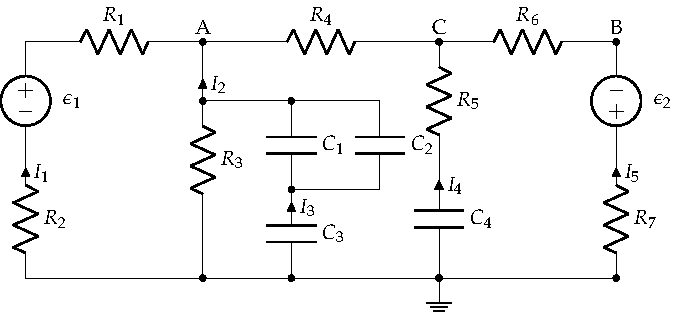
\includegraphics{figuras/mallas_agrupacion_condensadores.pdf}
\end{center}


\subsection*{Solución}
Se sustituyen los condensadores por circuitos abiertos. En
consecuencia, por las ramas correspondientes no puede circular
corriente. En particular:

\begin{align*}
  I_3 &= {0}{A}\\
  I_4 &= {0}{A}
\end{align*}

Se tienen entonces dos mallas. Definiendo dos corrientes de malla con
giro a derechas:

\begin{equation*}
  \begin{bmatrix}
    3 & -1\\
    -1 & 4\\
  \end{bmatrix} \cdot %
  \begin{bmatrix}
    I_a\\
    I_b
  \end{bmatrix} = %
  \begin{bmatrix}
    1\\
    7
  \end{bmatrix}
\end{equation*}

La solución de este sistema es:

\begin{align*}
  I_a &= {1}{A}\\
  I_b &= {2}{A}
\end{align*}
siendo,
\begin{align*}
  I_1 &= I_a = {1}{A}\\
  I_2 &= I_b - I_a = {1}{A}\\
  I_5 &= -I_b = {-2}{A}
\end{align*}

Se calcula ahora el balance de potencias, diferenciando entre
elementos activos (generadores) y pasivos (receptores):
\begin{itemize}
\item \textbf{Potencia de los generadores:}
  \begin{itemize}
  \item $P_{\epsilon1}=-\epsilon_1\,I_1=-1\cdot 1=-1$ W (G)
  \item $P_{\epsilon2}=\epsilon_2\,I_5=7\cdot (-2)=-14$ W (G)
  \end{itemize}
\item \textbf{Potencia de las resistencias:}
  \begin{itemize}
  \item $P_{R1}=R_1\,I_1^2=1\cdot 1^2=1$ W
  \item $P_{R2}=R_2\,I_1^2=1\cdot 1^2=1$ W
  \item $P_{R3}=R_3\,I_2^2=1\cdot 1^2=1$ W
  \item $P_{R4}=R_4\,(I_1+I_2)^2=1\cdot (1+1)^2=4$ W
  \item $P_{R5}=R_5\,I_4^2=1\cdot 0^2=0$ W
  \item $P_{R6}=R_6\,I_5^2=1\cdot (-2)^2=4$ W
  \item $P_{R7}=R_7\,I_5^2=1\cdot (-2)^2=4$ W
  \end{itemize}
\end{itemize}
cumpliéndose que $\sum P = 0$. Los potenciales en los puntos indicados
son:
\begin{align*}
  U_A &= -I_2 \cdot R_3 = -1\cdot 1= \qty{-1}{V}\\
  U_B &= -\epsilon_2 - I_5 \cdot R_7 =-7-(-2)\cdot 1= \qty{-5}{V}\\
  U_C &= U_{CB} + U_B = -I_5 \cdot R_6 + U_B = -(-2)\cdot 1+(-5)= \qty{-3}{V}
\end{align*}

La carga almacenada en el condensador $C_4$ se calcula con la
ecuación:
\begin{equation*}
  q_4 = C_4 \cdot U_{C4} = C_4 \cdot (-U_C) = \qty{12}{\micro\coulomb}
\end{equation*}
donde se ha asignado la polaridad positiva en la conexión a tierra.

Los condensadores $C_1$, $C_2$ y $C_3$ forman parte de una
asociación. Los condensadores $C_1$ y $C_2$ están asociados en
paralelo:
\begin{equation*}
  C_{12} = C_1 || C_2 = C_1 + C_2 = 1+2={3}{\mu F}
\end{equation*}
A su vez, están conectados en serie con el condensador $C_3$:
\begin{equation*}
  C_{eq} = \frac{C_{12} \cdot C_3}{C_{12} + C_3} =\dfrac{3\cdot 3}{3+3}= {1.5}{\mu F}
\end{equation*}
Este condensador equivalente está conectado entre A y tierra, y
asignando la polaridad positiva a la conexión a tierra:
\begin{equation*}
  U_{CT} = -U_A = {1}{V} \Rightarrow q_T = C_T \cdot U_{CT} =1.5\cdot 1= {1.5}{\mu F}
\end{equation*}
Al tratarse de una conexión serie, esta carga es la misma que tienen
el condensador $C_3$ y el condensador equivalente $C_{12}$.
\begin{align*}
  q_3 &=  {1.5}{\mu C}\\
  q_{12} &=  {1.5}{\mu C}
\end{align*}
Con estas cargas se puede calcular las diferencias de potencial en
estos condensadores:
\begin{align*}
  U_{C3} &=  \frac{q_3}{C_3} = \dfrac{1.5}{3}={0.5}{V}\\
  U_{C12} &=  \frac{q_{12}}{C_{12}}=\dfrac{1.5}{3} = {0.5}{V}
\end{align*}
Por tanto:
\begin{align*}
  q_1 &= C_1 \cdot U_{C12}=1\cdot 0.5 = {0.5}{\mu C}\\
  q_2 &= C_2 \cdot U_{C12}=2\cdot 0.5 = {1}{\mu C}
\end{align*}
donde se comprueba que $q_1 + q_2 = q_{12}$.

%%%%%%%%%%%%%%%%%%%%%%%%%%%%%%%%%%%%%%%%%%%%%%%%%%%%%%%%%%%%%%%%%%
\section{Enunciado}
El circuito de la figura está funcionando en régimen estacionario. Los
condensadores estaban inicialmente descargados. Resuelve el circuito
mediante el método que consideres conveniente para obtener los
siguientes resultados:
\begin{itemize}
\item Las intensidades señaladas.
\item Polaridad y energía almacenada en los condensadores.
\item Balance de potencias.
\end{itemize}
Datos:
$\epsilon_{1}={40}V; \epsilon_{2}={22}V; \epsilon_{3}={20}V;
C_{1}=C_{2}=C_{3}={2}{\mu F}; R_{g1}=R_{g2}=R_{g3}={4}{\Omega};
R_{1}=R_{2}=R_{3}=R_{4}={2}{\Omega}; R_{5}=R_{6}=R_{7}={1}{\Omega}$

\begin{center}
  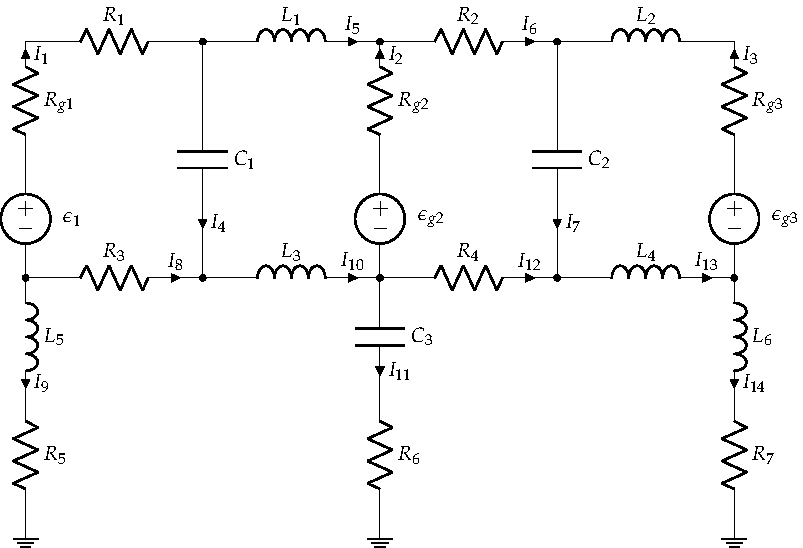
\includegraphics{figuras/mallas_condensadores_bobinas.pdf}
\end{center}


\subsection*{Solución}
Los condensadores se sustituyen por circuitos abiertos (inicialmente
están descargados) y las bobinas por cortocircuitos. De esta forma, el
circuito original queda reducido a tres mallas, como se muestra en la
siguiente figura:

\begin{center}
  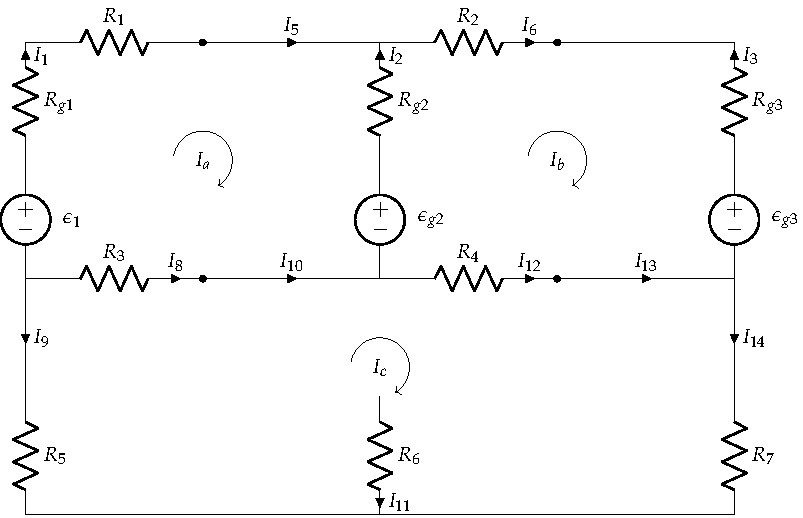
\includegraphics{figuras/mallas_condensadores_bobinas_mod.pdf}
\end{center}


Se resuelve mediante el método de mallas, cuyo sistema de ecuaciones
en forma matricial es:
\begin{equation*}
  \begin{bmatrix}
    12 & -4 & -2 \\
    -4 & 12 & -2\\
    -2 & -2 & 6
  \end{bmatrix}
  \cdot\begin{bmatrix}
         I_a\\
         I_b\\
         I_c
       \end{bmatrix}
       =
       \begin{bmatrix}
         18\\
         2\\
         0
       \end{bmatrix}
     \end{equation*}
     cuya solución es:
     \begin{align*}
       I_{a} & =  2\, A\\
       I_{b} & =  1\, A\\
       I_{c} & =  1\, A
     \end{align*}
     Relacionando estas corrientes de malla con las corrientes de rama
     señaladas en el circuito original (teniendo en cuenta que las
     corrientes que circulan por ramas con condensadores son nulas):
     \begin{align*}
       I_{1} & =  I_{a}=2\, A\\
       I_{2} & =  -I_{a}+I_{b}=-1\, A\\
       I_{3} & =  -I_{b}=-1\, A\\
       I_{4} & =  0\, A\\
       I_{5} & =  I_{a}=2\, A\\
       I_{6} & =  I_{b}=1\, A\\
       I_{7} & =  0\, A\\
       I_{8} & =  -I_{a}+I_{c}=-1\, A\\
       I_{9} & =  -I_{c}=-1\, A\\
       I_{10} & = -I_{a}+I_{c}=-1\, A\\
       I_{11} & =  0\, A\\
       I_{12} & =  -I_{b}+I_{c}=0\, A\\
       I_{13} & =  -I_{b}+I_{c}=0\, A\\
       I_{14} & =  I_{c}=1\, A
     \end{align*}

     El condensador $C_{1}$ está conectado directamente a la rama
     compuesta por la fuente $E_{2}$ y su resistencia $E_{g2}$ (debido
     a que la bobina se comporta como un cortocircuito). Por tanto,
     suponiendo que la polaridad positiva de este condensador
     corresponde a su borne superior, la tensión de este condensador
     es:
     \begin{equation*}
       U_{C1}=E_{2}-I_{2}\cdot R_{g2}=22-(-1)\cdot4=26\, V
     \end{equation*}
     siendo correcta la polaridad asignada por el signo positivo de
     este resultado. La energía almacenada por el condensador es:
     \begin{equation*}
       E_{C1}=1/2\cdot V_{c1}^{2}\cdot C_{1}=0.676\, mJ
     \end{equation*}

     El condensador $C_{2}$ está conectado directamente a la rama
     compuesta por la fuente $E_{3}$ y su resistencia $E_{g3}$ (debido
     a que la bobina se comporta como un cortocircuito). Por tanto,
     suponiendo que la polaridad positiva de este condensador
     corresponde a su borne superior, la tensión de este condensador
     es:
     \begin{equation*}
       U_{C2}=E_{3}-I_{3}\cdot R_{g3}=20-(-1)\cdot4=24\, V
     \end{equation*}
     siendo correcta la polaridad asignada por el signo positivo de
     este resultado. La energía almacenada por el condensador es:
     \begin{equation*}
       E_{C2}=1/2\cdot U_{C2}^{2}\cdot C_{2}=0.576\, mJ
     \end{equation*}

     El condensador $C_{3}$ está en paralelo con la resistencia
     $R_{4}$ y la resistencia $R_{7}$ (debido a que las bobinas se
     comportan como un cortocircuito y a que por la resistencia
     $R_{6}$ no circula corriente). Por tanto, suponiendo que la
     polaridad positiva de este condensador corresponde a su borne
     superior, la tensión de este condensador es:
     \begin{equation*}
       U_{C3}=I_{12}\cdot R_{4}+I_{14}\cdot R_{7}=0+1\cdot1=1\, V
     \end{equation*}
     siendo correcta la polaridad asignada por el signo positivo de
     este resultado. La energía almacenada por el condensador es:
     \begin{equation*}
       E_{C3}=1/2\cdot U_{C3}^{2}\cdot C_{3}=1\,\mu J
     \end{equation*}

     Se calcula ahora el balance de potencias, diferenciando entre
     elementos activos (generadores) y pasivos (receptores):
     \begin{itemize}
     \item \textbf{Potencia de los generadores:}
       \begin{itemize}
       \item $P_{\epsilon1}=-\epsilon_1\,I_1=-40\cdot 2=-80$ W (G)
       \item $P_{\epsilon2}=-\epsilon_2\,I_2=-22\cdot (-1)=22$ W (R)
       \item $P_{\epsilon3}=-\epsilon_3\,I_3=-20\cdot (-1)=20$ W (R)
       \end{itemize}
     \item \textbf{Potencia de las resistencias:}
       \begin{itemize}
       \item $P_{Rg1}=R_{g1}\,I_1^2=4\cdot 2^2=16$ W
       \item $P_{Rg2}=R_{g2}\,I_2^2=4\cdot (-1)^2=4$ W
       \item $P_{Rg3}=R_{g3}\,I_3^2=4\cdot (-1)^2=4$ W
       \item $P_{R1}=R_1\,I_1^2=2\cdot 2^2=8$ W
       \item $P_{R2}=R_2\,I_6^2=2\cdot 1^2=2$ W
       \item $P_{R3}=R_3\,I_8^2=2\cdot (-1)^2=2$ W
       \item $P_{R4}=R_4\,I_{12}^2=2\cdot 0^2=0$ W
       \item $P_{R5}=R_5\,I_9^2=1\cdot (-1)^2=1$ W
       \item $P_{R6}=R_6\,I_{11}^2=1\cdot 0^2=0$ W
       \item $P_{R7}=R_7\,I_{14}^2=1\cdot 1^2=1$ W
       \end{itemize}
     \end{itemize}
     cumpliéndose que $\sum P = 0$.

%%%%%%%%%%%%%%%%%%%%%%%%%%%%%%%%%%%%%%%%%%%%%%%%%%%%%%%%%%%%%%%%%%
     \section{Enunciado}
     En el circuito de la figura, obtener las intensidades de
     corriente señaladas mediante un análisis por el método de las
     mallas y mediante un análisis por el método de los nudos.

     \begin{center}
       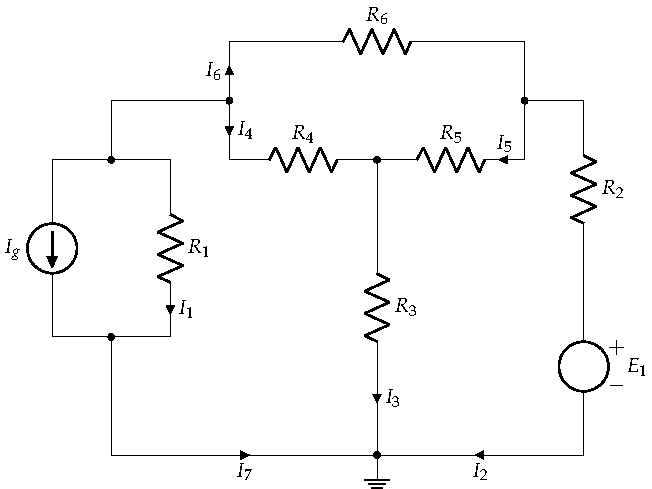
\includegraphics{figuras/BT1_12.pdf}
     \end{center}

     \subsection*{Solución}

     \textbf{Resolución mediante mallas}

     Se hace la transformación de la fuente de corriente en una fuente
     de tensión:
     \begin{equation*}
       \epsilon_{Ig}=I_g\cdot R_9=2\cdot 9=18\,V
     \end{equation*}
     Así, el circuito está formado por 3 mallas como se muestra en la
     figura:
     \begin{center}
       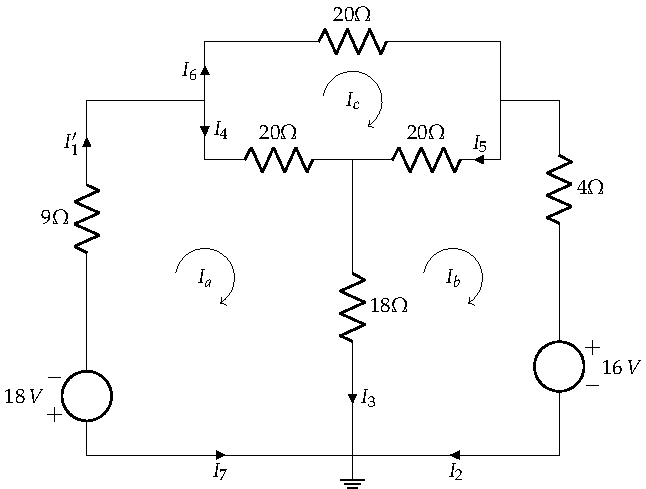
\includegraphics{figuras/BT1_12_mallas.pdf}
     \end{center}
     
     Se plantea el sistema en forma matricial:
     \begin{equation*}
       \begin{bmatrix}
         47 & -18 & -20\\
         -18 & 42 & -20\\
         -20 & -20 & 60
       \end{bmatrix}
       \cdot
       \begin{bmatrix}
         I_a\\
         I_b\\
         I_c
       \end{bmatrix}
       =
       \begin{bmatrix}
         -18\\
         -16\\
         0
       \end{bmatrix}
     \end{equation*}
     cuya solución es:
     \begin{align*}
       I_a&=\qty{-1.26}{\ampere}\\
       I_b&=\qty{-1.33}{\ampere}\\
       I_c&=\qty{-0.87}{\ampere}\\
     \end{align*}
     Estableciendo las relaciones con las corrientes de rama
     indicadas:
     \begin{align*}
       I_1'&=I_a=\qty{-1.26}{\ampere}\\
       I_2&=I_b=\qty{-1.33}{\ampere}\\
       I_3&=I_a-I_b=-1.26-(-1.33)=\qty{0.07}{\ampere}\\
       I_4&=I_a-I_c=-1.26-(-0.87)=\qty{-0.39}{\ampere}\\
       I_5&=I_c-I_b=-0.87-(-1.33)=\qty{0.46}{\ampere}\\
       I_6&=I_c=\qty{-0.87}{\ampere}\\
       I_7&=-I_a=\qty{1.26}{\ampere}\\
     \end{align*}
     La corriente $I_1$ del circuito original se obtiene aplicando el
     1LK:
     \begin{equation*}
       I_g+I_1=I_7\Rightarrow I_1=I_7-I_g=1.26-2=\qty{-0.74}{\ampere}
     \end{equation*}

     \textbf{Resolución mediante nudos}

     Se transforma la fuente de tensión en una de corriente:
     \begin{equation*}
       I_{\epsilon,g}=\dfrac{\epsilon_g}{R_4}=\dfrac{16}{4}=\qty{4}{\ampere}
     \end{equation*}
     quedando el circuito que se muestra en la figura:
     \begin{center}
       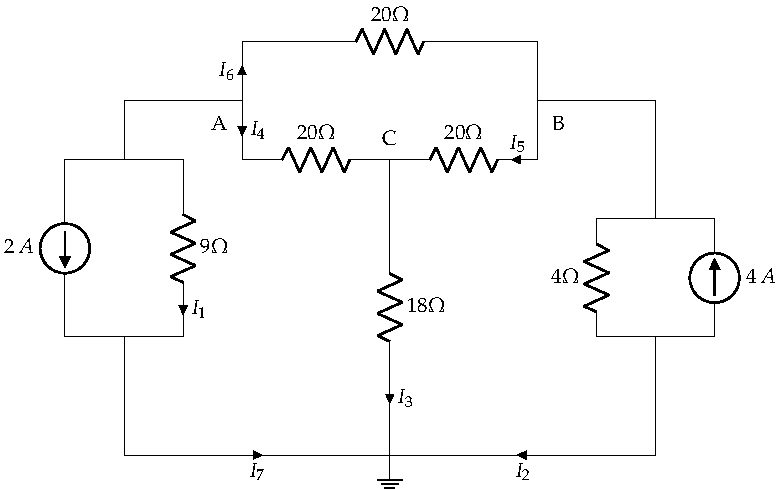
\includegraphics{figuras/BT1_12_nudos.pdf}
     \end{center}
     Con los nudos indicados, se aplica el método de nudos en su forma
     matricial:
     \begin{equation*}
       \begin{bmatrix}
         \dfrac{19}{90} & -\dfrac{1}{20} & -\dfrac{1}{20}\\[10pt]
         -\dfrac{1}{20} & \dfrac{7}{20} & -\dfrac{1}{20}\\[10pt]
         -\dfrac{1}{20} & -\dfrac{1}{20} & \dfrac{7}{45}
       \end{bmatrix}
       \cdot
       \begin{bmatrix}
         U_A\\
         U_B\\
         U_C
       \end{bmatrix}
       =
       \begin{bmatrix}
         -2\\
         4\\
         0
       \end{bmatrix}
     \end{equation*}
     cuya solución es:
     \begin{align*}
       U_A&=-6.64\,V\\
       U_B&=10.66\,V\\
       U_C&=1.29\,V\\
     \end{align*}
     A partir de 1LK, 2LK y ley de Ohm, se obtienen las corrientes
     indicadas:
     \begin{align*}
       I_1&=\dfrac{U_A}{R_9}=\dfrac{-6.64}{9}=\qty{-0.74}{\ampere}\\[7pt]
       I_2&= I_{R_4}-I_{\epsilon,g}=\dfrac{U_B}{R_4}-4=\dfrac{10.66}{4}-4=\qty{-1.34}{\ampere}\\[7pt]
       I_3&=\dfrac{U_C}{R_{18}}=\dfrac{1.29}{18}=\qty{0.07}{\ampere}\\[7pt]
       I_4&=\dfrac{U_{AC}}{R_{20}}=\dfrac{U_A-U_C}{R_{20}}=\dfrac{-6.64-1.29}{20}=\qty{-0.39}{\ampere}\\[7pt]
       I_5&=\dfrac{U_{BC}}{R_{20}}=\dfrac{U_B-U_C}{R_{20}}=\dfrac{10.66-1.29}{20}=\qty{0.47}{\ampere}\\[7pt]
       I_6&=\dfrac{U_{AB}}{R_{20}}=\dfrac{U_A-U_B}{R_{20}}=\dfrac{-6.64-10.66}{20}=\qty{-0.87}{\ampere}\\[7pt]
       I_7&=I_g+I_1
     \end{align*}

     Se observa que los valores obtenidos son idénticos con ambos
     métodos.
%%%%%%%%%%%%%%%%%%%%%%%%%%%%%%%%%%%%%%%%%%%%%%%%%%%%%%%%%%%%%%%%%%
     \section{Enunciado}
     Calcular la intensidad que circula por la resistencia de 30
     $\Omega$ del circuito de la figura aplicando el principio de
     superposición.

\begin{center}
  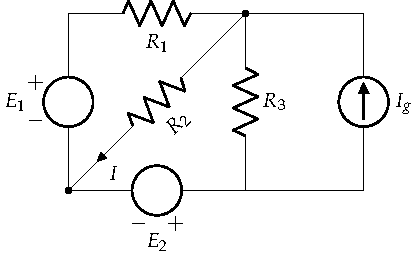
\includegraphics[width=0.35\linewidth]{figuras/BT1_16.pdf}
\end{center}

\subsection*{Solución}
El circuito es equivalente a la suma de tres circuitos en los que
únicamente aparece un generador, anulándose el resto (cortocircuitando
la fuente de tensión y dejando en circuito abierto la fuente de
corriente). Se analiza cada circuito por separado.

\textbf{Actúa solo la fuente de tensión de 32 V}

Las resistencia equivalente del paralelo es:
\begin{equation*}
  R_{paralelo}=\dfrac{20\cdot 30}{20+30}=12\Omega
\end{equation*}
siendo la corriente total del circuito, por ley de Ohm:
\begin{equation*}
  I=\dfrac{32}{20+12}=\qty{1}{\ampere}
\end{equation*}
Con el concepto de divisor de corriente, la corriente $I'$ (la que
circula por la resistencia de 30 $\Omega$ en este caso) es:
\begin{equation*}
  I'=I\cdot \dfrac{R_{paralelo}}{R}=1\cdot\dfrac{12}{30}=\qty{0.4}{\ampere}
\end{equation*}

\textbf{Actúa solo la fuente de tensión de 64 V}

Las resistencia equivalente del paralelo es:
\begin{equation*}
  R_{paralelo}=\dfrac{20\cdot 30}{20+30}=12\Omega
\end{equation*}
siendo la corriente total del circuito, por ley de Ohm:
\begin{equation*}
  I=\dfrac{64}{20+12}=\qty{2}{\ampere}
\end{equation*}
Con el concepto de divisor de corriente, la corriente $I''$ (la que
circula por la resistencia de 30 $\Omega$ en este caso) es:
\begin{equation*}
  I''=I\cdot \dfrac{R_{paralelo}}{R
  }=2\cdot\dfrac{12}{30}=\qty{0.8}{\ampere}
\end{equation*}

\textbf{Actúa solo la fuente de corriente de 4 A}

Las resistencia equivalente del circuito es (las tres están en
paralelo):
\begin{equation*}
  R_{eq}=\dfrac{1}{\frac{1}{20}+\frac{1}{20}+\frac{1}{30}}=7.5\Omega
\end{equation*}

Dado que la corriente total del circuito son 4 A, con el concepto de
divisor de corriente, la corriente $I'''$ (la que circula por la
resistencia de 30 $\Omega$ en este caso) es:
\begin{equation*}
  I'''=I\cdot \dfrac{R_{eq}}{R}=4\cdot\dfrac{7.5}{30}=\qty{1}{\ampere}
\end{equation*}

Por tanto, la corriente total que circula por la resistencia de
$30\Omega$ es:
\begin{equation*}
  I=I'+I''+I'''=0.4+0.8+1=\qty{2.2}{\ampere}
\end{equation*}

%%%%%%%%%%%%%%%%%%%%%%%%%%%%%%%%%%%%%%%%%%%%%%%%%%%%%%%%%%%%%%%%%%
\section{Enunciado}
Obtener el generador equivalente de Thévenin del circuito de la figura
respecto de A y B. A partir de este generador, calcula la resistencia
a colocar en AB para obtener la máxima potencia, calculando esta
potencia y la potencia entregada por el generador $\epsilon$.

Datos:
$\epsilon = \qty{54}{\volt};\quad R_1 = R_4 = \qty{8}{\ohm};\quad R_2
= R_3 = \qty{10}{\ohm}$

\begin{center}
  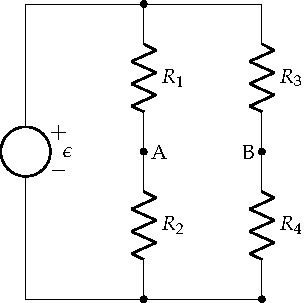
\includegraphics{figuras/Thevenin2}
\end{center}

    
\subsection*{Solución}
Para obtener la tensión $U_{AB}$ aplicamos divisor de tensión en ambas
ramas:

\begin{align*}
  U_A &= \epsilon \cdot \frac{R_2}{R_1 + R_2}\\
  U_B &= \epsilon \cdot \frac{R_4}{R_3 + R_4}\\
  U_{AB} &= \epsilon \cdot (\frac{R_2}{R_1 + R_2} -  \frac{R_4}{R_3 + R_4}) = \SI{6}{\volt} = \epsilon_{th}
\end{align*}

Para calcular la resistencia equivalente apagamos la fuente de
tensión. En el circuito resultante obtenemos:

\begin{equation*}
  R_{th} = (R_1 || R_2) + (R_3 || R_4) = 80/9\si{\ohm}
\end{equation*}

Para obtener la máxima potencia hay que conectar una resistencia
$R_L = R_{th}$. Con esta resistencia el balance de potencias es:

\begin{align*}
  P_L &= \frac{\epsilon_{th}^2}{4R_{th}} = \SI{1.0125}{\watt}\\
  P_\epsilon &= 2 \cdot P_L = \SI{2.025}{\watt}
\end{align*}

%%%%%%%%%%%%%%%%%%%%%%%%%%%%%%%%%%%%%%%%%%%%%%%%%%%%%%%%%%%%%%%%%% 

\section{Enunciado}
Determinar el equivalente Thévenin del circuito de la figura entre los
nudos $A-B$. ¿Qué resistencia habría que conectar en dichos terminales
para transferir la máxima potencia? ¿Cuál sería dicha potencia?

\begin{center}
  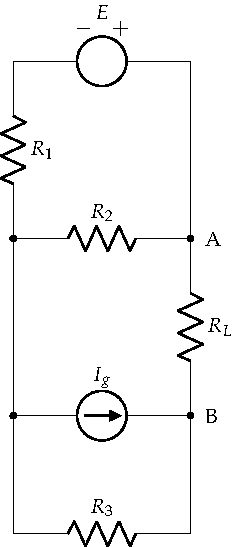
\includegraphics{figuras/BT1_17.pdf}
\end{center}

\subsection*{Solución}
Se transforma la fuente de corriente en paralelo con la resistencia de
$2\Omega$ en una fuente de tensión en serie con dicha resistencia,
como en la Figura~\ref{fig.BT1_17_mallas}:
\begin{equation*}
  U_{I_g}=I_g\cdot R_2=8\cdot 2=16\, V
\end{equation*}

\begin{center}
  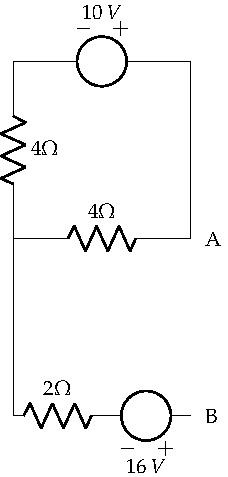
\includegraphics{figuras/BT1_17_mallas.pdf}
\end{center}


\textbf{Cálculo de $\epsilon_{th}$}

Hay que determinar la tensión $U_{AB}$. Considerando el nudo de la
izquierda como masa, y dado que por la resistencia de $2\Omega$ no
circula corriente (circuito abierto entre $A-B$), la tensión en $B$
es:
\begin{equation*}
  U_B=16\,V
\end{equation*}
Aplicando la ley de Ohm a la malla superior:
\begin{equation*}
  I=\dfrac{10}{4+4}=\qty{1.25}{\ampere}
\end{equation*}
por lo que la tensión en el punto $A$:
\begin{equation*}
  U_A=4\cdot 1.25=5\,V
\end{equation*}
Así, la tensión $U_{AB}=\epsilon_{th}$:
\begin{equation*}
  U_{AB}=U_A-U_B=\epsilon_{th}=5-16=-11\,V
\end{equation*}

\textbf{Cálculo de $R_{th}$}

Al no haber fuentes dependientes, se puede obtener esta resistencia
como la $R_{eq}$ vista desde los terminales $A-B$, anulando las
fuentes:
\begin{equation*}
  R_{eq}=R_{th}=2+\dfrac{4\cdot 4}{4+4}=4\Omega
\end{equation*}

\textbf{Equivalente Thévenin} El equivalente de Thévenin queda como se
muestra a continuación:

\begin{center}
  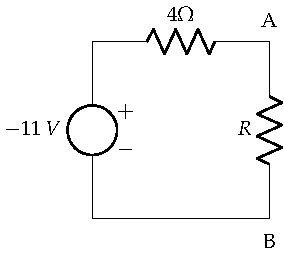
\includegraphics{figuras/BT1_17_th.pdf}
\end{center}

Aplicando el T. Máx. Trans. Potencia, la resistencia a conectar es:
\begin{equation*}
  R_L=R_{th}=4\Omega
\end{equation*}
siendo la máxima potencia transferida:
\begin{equation*}
  P_{max}=\dfrac{\epsilon_{th}^2}{4\,R_{th}}=\dfrac{(-11)^2}{4\cdot 4}=7.56\,W
\end{equation*}

%%%%%%%%%%%%%%%%%%%%%%%%%%%%%%%%%%%%%%%%%%%%%%%%%%%%%%%%%%%%%%%%%%

\section{Enunciado}
Obtener el generador equivalente de Thévenin del circuito de la Figura~\ref{fig.BT1_18} respecto de A y B.\\
Datos: $I_g=\qty{10}{\ampere}; R_1=1\Omega;\; \alpha=5$
\begin{center}
  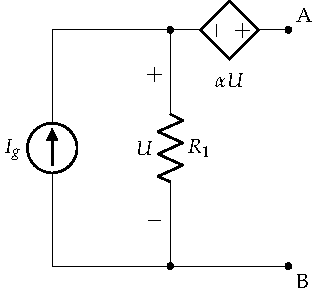
\includegraphics{figuras/Thevenin1.pdf}
\end{center}

\subsection*{Solución}
Por una parte:
\begin{equation*}
  U_{AB} = \alpha U + U = (1 + \alpha) U=(1+5)U=6\,U
\end{equation*}
Además:
\begin{equation*}
  U = I_g \cdot R_1=10\cdot 1 = 10\,V
\end{equation*}
Por tanto, el generador de Thévenin tiene una fem de:
\begin{equation*}
  U_{AB} = 6\, U= 6\cdot 10=60 V = \epsilon_{th}
\end{equation*}

Para calcular la impedancia, se apaga la fuente independiente. Como la
fuente dependiente permanece, es necesario aplicar un generador de
prueba a la salida:

\begin{center}
  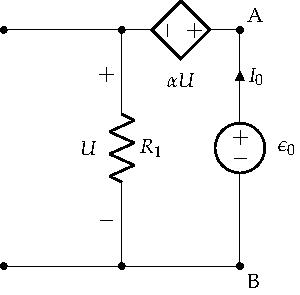
\includegraphics{figuras/Thevenin1_fuenteprueba.pdf}
\end{center}

\begin{align*}
  \epsilon_0 &= \alpha U + U = U(1+\alpha)=6\,U\\
  U &= I_0\,R_1=I_0\cdot 1=I_0
\end{align*}
Por tanto,

\begin{equation*}
  R_{th} = \dfrac{\epsilon_0}{I_0}=\dfrac{6\,U}{U} = 6 \Omega
\end{equation*}

%%%%%%%%%%%%%%%%%%%%%%%%%%%%%%%%%%%%%%%%%%%%%%%%%%%%%%%%%%%%%%%%%%

\section{Enunciado}

En el circuito de la figura, calcular:
\begin{itemize}
\item La corriente del generador equivalente de Norton respecto de A y
  B, $I_N$.
\item La resistencia del generador equivalente de Norton respecto de A
  y B, $R_N$.
\item La resistencia de carga que se debe conectar entre A y B para
  conseguir la máxima potencia disponible, y el valor de esta
  potencia.
\end{itemize}

Datos: $R = {1}{\Omega};\; \epsilon_g = {10}{V};\; \alpha = \beta = 1$

\begin{center}
  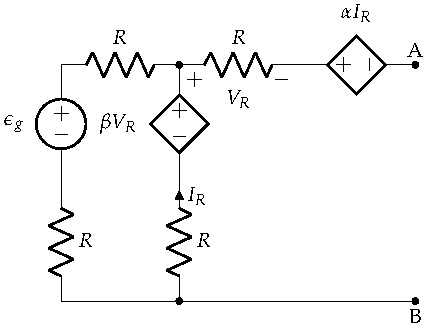
\includegraphics{figuras/norton.pdf}
\end{center}

\subsection*{Solución}
Para calcular el equivalente de Norton, se cortocircuita la salida del
circuito:
\begin{center}
  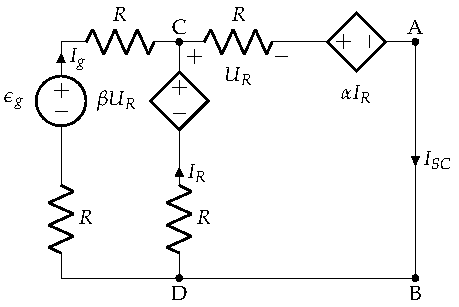
\includegraphics{figuras/norton_corto.pdf}
\end{center}

Aplicando el método de mallas, ambas en sentido horario:
\begin{equation*}
  \begin{bmatrix}
    3 & -1\\
    -1 & 2
  \end{bmatrix}
  \cdot 
  \begin{bmatrix}
    I_a\\
    I_b
  \end{bmatrix}
  = 
  \begin{bmatrix}
    10-1\,U_R\\
    1\,U_R-1\,I_R
  \end{bmatrix}
\end{equation*}
donde además se sabe que:
\begin{align*}
  I_R&=I_b-I_a\\
  U_R&=1\, I_b
\end{align*}
Combinando las ecuaciones, se obtiene que:
\begin{equation*}
  I_a=I_b=I_{sc}=\dfrac{10}{3}\,A
\end{equation*}
    
Para obtener la resistencia equivalente, se apaga la fuente
independiente y se conecta un generador de prueba en AB:
\begin{center}
  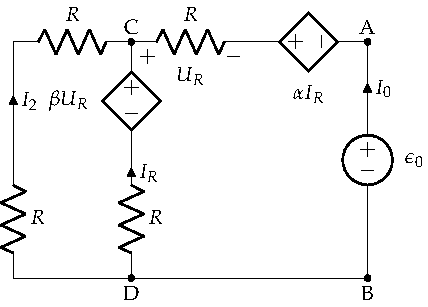
\includegraphics{figuras/norton_fuenteprueba.pdf}
\end{center}


Aplicando el método de mallas, ambas en sentido horario:
\begin{equation*}
  \begin{bmatrix}
    3 & -1\\
    -1 & 2
  \end{bmatrix}
  \cdot 
  \begin{bmatrix}
    I_a\\
    I_b
  \end{bmatrix}
  = 
  \begin{bmatrix}
    -1\,U_R\\
    1\,U_R-1\,I_R-\epsilon_0
  \end{bmatrix}
\end{equation*}
donde además se sabe que:
\begin{align*}
  I_R&=I_b-I_a\\
  U_R&=1\, I_b
\end{align*}
Combinando las ecuaciones, se obtiene que:
\begin{align*}
  I_a&=\qty{0}{\ampere}\\
  I_b&=-\dfrac{\epsilon_0}{2}
\end{align*}
y, dado que:
\begin{equation*}
  I_0=-I_b=\dfrac{\epsilon_0}{2}
\end{equation*}
la resistencia de Norton:
\begin{equation*}
  R_{N} = \dfrac{\epsilon_0}{I_0}=\dfrac{\epsilon_0}{\frac{\epsilon_0}{2}} = {2}{\Omega}
\end{equation*}

Por tanto, habrá que conectar una resistencia de ${2}{\Omega}$ para
obtener la máxima potencia disponible, siendo entonces la potencia:
\begin{equation*}
  P_L=\dfrac{\epsilon_{th}^2}{4\,R_L}=\dfrac{(I_N\,R_N)^2}{4\,R_L}=\dfrac{(\frac{10}{3}\cdot 2)^2}{4\cdot 2}=5.56\,W
\end{equation*}

%%%%%%%%%%%%%%%%%%%%%%%%%%%%%%%%%%%%%%%%%%%%%%%%%%%%%%%%%%%%%%%%%%

% \section{Enunciado}
% Determinar las corrientes marcadas en la figura.
% \begin{center}
%   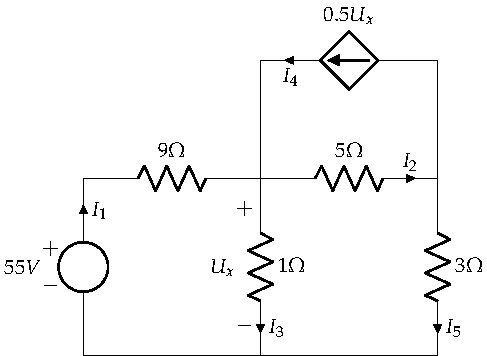
\includegraphics[width=0.45\linewidth]{figuras/BT1_13.pdf}
% \end{center}

% \subsection*{Solución}
% En primer lugar, se transforma la fuente de corriente dependiente de
% tensión en una fuente de tensión dependiente de tensión:
% \begin{equation*}
%   \epsilon_{I_g}=I_g\,R_{5}=0.5\, U_x\cdot 5=2.5\,U_x
% \end{equation*}
% Con esta transformación, se aplica el método de mallas como se muestra
% a continuación:

% \begin{center}
%   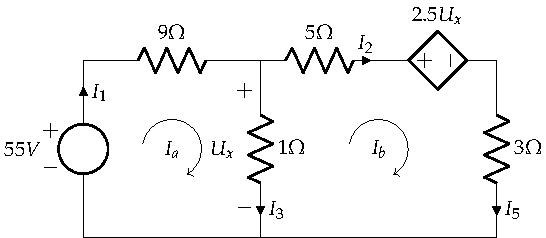
\includegraphics{figuras/BT1_13_mallas.pdf}
% \end{center}

% Se plantea el sistema de ecuaciones en forma matricial:
% \begin{equation*}
%   \begin{bmatrix}
%     10 & -1\\
%     -1 & 9
%   \end{bmatrix}
%   \cdot 
%   \begin{bmatrix}
%     I_a\\
%     I_b
%   \end{bmatrix}
%   =
%   \begin{bmatrix}
%     55\\
%     -2.5\,U_x
%   \end{bmatrix}
% \end{equation*}
% donde se sabe además que $U_x=R_1\, I_3=1\,(I_a-I_b)$. Resolviendo el
% sistema de 3 ecuaciones con 3 incógnitas, se obtiene que:
% \begin{align*}
%   I_a&= \qty{5.38}{\ampere}\\
%   I_b&= \qty{-1.24}{\ampere}
% \end{align*}
% siendo las corrientes de rama:
% \begin{align*}
%   I_1&=I_a=\qty{5.38}{\ampere}\\
%   I_3&=I_a-I_b=5.38-(-1.24)=\qty{6.62}{\ampere}\\
%   I_5&=I_b=\qty{-1.24}{\ampere}
% \end{align*}
% La corriente $I_4$ del circuito original se obtiene a partir de $U_x$:
% \begin{equation*}
%   I_4=0.5\,U_x=0.5\, R_1\, I_3=0.5\cdot 1 \cdot 6.62=\qty{3.31}{\ampere}
% \end{equation*}
% e $I_2$ se obtiene con la 1LK:
% \begin{equation*}
%   I_1+I_4=I_2+I_3\Rightarrow I_2=I_1+I_4-I_3=5.38+3.31-6.62=\qty{2.07}{\ampere}
% \end{equation*}
 
% %%%%%%%%%%%%%%%%%%%%%%%%%%%%%%%%%%%%%%%%%%%%%%%%%%%%%%%%%%%%%%%%%%
  
% \section{Enunciado}

% Determinar las tensiones en los nudos $A$ y $B$ del circuito de la
% figura.
% \begin{center}
%   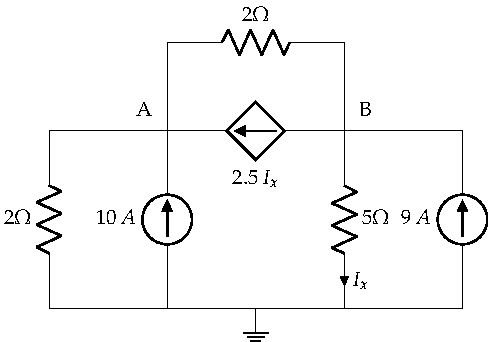
\includegraphics[]{figuras/BT1_14.pdf}
% \end{center}

% \subsection*{Solución}
% Se resuelve mediante el método de nudos. El sistema de ecuaciones en
% forma matricial es:
% \begin{equation*}
%   \begin{bmatrix}
%     \dfrac{1}{2}+\dfrac{1}{2} & -\dfrac{1}{2}\\[10pt]
%     -\dfrac{1}{2} & \dfrac{1}{2}+\dfrac{1}{5}
%   \end{bmatrix}
%   \cdot
%   \begin{bmatrix}
%     U_a\\
%     U_b
%   \end{bmatrix}
%   =
%   \begin{bmatrix}
%     10+2.5\,I_x\\
%     9-2.5\,I_x
%   \end{bmatrix}
% \end{equation*}
% donde se sabe, además, que
% $I_x=\dfrac{U_b}{R_5}=\dfrac{U_b}{5}$. Resolviendo el sistema, se
% obtiene que:
% \begin{align*}
%   U_a&=30\,V\\
%   U_b&=20\,V
% \end{align*}
 

%%% Local Variables:
%%% mode: latex
%%% TeX-master: "Problemas_TC"
%%% ispell-local-dictionary: "castellano"
%%% End:

